\subsection{Leapfrog algorithm}
The leapfrog algorithm, given by the update rule \cite{young_leapfrog_2019}
\begin{equation}\label{eq:leapfrog}
    \begin{aligned}
        \mathbf{v}_{i}^{(1/2)} & = \mathbf{v}_i^{(0)} + \frac{1}{2}\textrm{DT} \frac{\mathbf{F}_i^{(0)}}{ m_i^{(0)}}, \\
        \mathbf{x}_i^{(k+1)}   & = \mathbf{x}_i^{(k)} + \textrm{DT} \mathbf{v}_i^{(k+1/2)},                           \\
        \mathbf{v}_i^{(k+3/2)} & = \mathbf{v}_i^{(k+1/2)} + \textrm{DT} \frac{ \mathbf{F}_i^{(k+1)}}{m_i}.
    \end{aligned}
\end{equation}
is the preferred way of integrating \autoref{eq:newtons-second}.
When applied to the same pendulum system, it conserves energy much more faithfully and preserves the area in phase space, consistent with Liouville's theorem (see \autoref{fig:leapfrog-integrator} and \autoref{fig:area-euler-vs-leapfrog}).
\begin{figure}[htp]
    \centering
    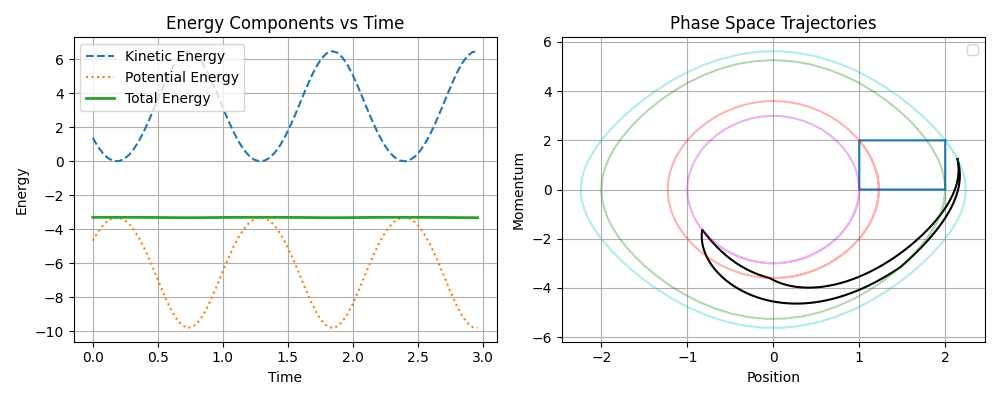
\includegraphics[scale=0.6]{img/integrators/leapfrog-pendulum.png}
    \caption{Behavior of the leapfrog algorithm: conservation of energy and phase space trajectories forming closed loops.
        Evolution of an area element in phase space is shown on the right-hand side: blue rectangle -- initial conditions for many copies of the system; black distorted quadrilateral -- their state by the end of the simulation.}
    \label{fig:leapfrog-integrator}
\end{figure}
Given its simplicity and excellent long-term energy behavior, we adopt the leapfrog algorithm to integrate Newton's equations in our program.